%===========================================================
%                              Choix: RenPar / SympA / CFSE
%===========================================================
% Une des trois options 'renpar', 'sympa' et 'cfse' doit
% être utilisée avec le style compas2013 en fonction 
% de l'appel à soumission choisi.
\documentclass[renpar]{compas2013}

\usepackage{verbatim}
\usepackage[french]{algorithm2e}

%===========================================================
%                        Title
%===========================================================

\toappear{1} % Conserver cette ligne pour la version finale

\begin{document}

\title{Optimisation du produit matrice-vecteur creux sur architecture GPU pour un simulateur de réservoir}
\shorttitle{SpMV sur GPU}

\author{Corentin Rossignon\thanks{Doctorant CIFRE, Total - Inria Bordeaux - LaBRI, Université Bordeaux 1, 351 cours de la libération, 33405 Talence. Le texte a été relu par Pascal Henon (Total), Olivier Aumage (Inria) et Samuel Thibault (Inria).}}%

\address{Total CSTJF - PAU\\
Avenue Larribau\\
64000 Pau - France\\
Corentin.Rossignon@Total.com}
%--------\\
%Inria Bordeaux - Sud-Ouest, LaBRI\\
%Equipe-projet Runtime\\
%Université Bordeaux 1\\
%351 cours de la libération\\
%33405 Talence\\
%Corentin.Rossignon@Inria.fr}

\date{01 décembre 2012}

\maketitle

%===========================================================
%                       Résumé
%===========================================================
\begin{abstract}
  Pour l'entreprise Total, la simulation de réservoir est une étape importante
  dans le processus d'optimisation de la production. Actuellement ces simulations
  s'exécutent entièrement sur CPU. Nous avons donc essayé d'accélérer les produits
  matrice-vecteur creux contenus dans le simulateur en utilisant des GPUs.
  Les bibliothèques GPU d'algèbre linéaire creux utilisent des formats génériques de stockage 
  de matrices creuses qui sont plus ou moins performant sur GPU mais qui ne
  permettent pas d'exploiter la structure
  particulière des matrices utilisées dans le simulateur de réservoir.
  Pour exploiter cette structure, nous avons adapté pour nos matrices un format de stockage
  qui nous permet d'accélérer jusqu'à un facteur 20 le produit
  matrice-vecteur creux sur 3 GPUs par rapport à 8 coeurs CPU et d'un facteur 1,5 sur GPU
  par rapport aux formats génériques utilisée par NVIDIA dans cuSPARSE.

  %% Max 5 mots clés
  \MotsCles{solveur creux, GPU, SpMV, CSR}
\end{abstract}


%=========================================================
\section{Introduction}
%=========================================================
 La simulation de réservoir (réserve naturelle d'hydrocarbures) est l'élément
 central dans l'étude des champs pétrolifères ou gaziers. Elle permet d'optimiser
 le placement des puits d'extraction, de calculer le rendement en hydrocarbures et aussi
 d'expérimenter de nouvelles méthodes d'extraction.
 
 Dans cette simulation, le temps est discrétisé avec un pas de l'ordre de la journée.
 Chaque pas nécessite de résoudre plusieurs systèmes d'équations linéaires.
 Ces résolutions représentent près de 70\% du temps de calcul utilisé
 par le simulateur.
 
 Actuellement ces simulations sont réalisées sur CPU, et le calcul est distribué avec MPI.
 L'émergence des solutions GPGPU et la promesse de performances font que le simulateur
 pourrait gagner à être porté sur GPU. La résolution de ces systèmes d'équations requiert
 l'utilisation de matrices creuses de grandes tailles. Pour réduire les ressources (CPU, RAM)
 utilisées par ces
 matrices, seuls les éléments non nuls des matrices sont stockés et leurs coordonnées
 peuvent être encodées de manière plus ou moins direct sous la forme d'un format de
 stockage.

 Sur GPU, ces formats de stockage auront un impact sur les performances,
 l'ordre des accès mémoire change en fonction du format et le GPU est
 un processeur sensible à l'ordre des accès mémoire.


%=========================================================
\section{Contexte}
%=========================================================
 %-------------------------------
 \subsection{Simulation de réservoir} 
  Dans la simulation de réservoir, le temps est discrétisé avec un pas
  de l'ordre de la journée. Pour
  chaque pas, il est nécessaire de faire converger un système
  non-linéaire, pour cela de nombreux systèmes linaires creux doivent
  être résolus. Les méthodes de résolution de systèmes linaires creux
  utilisent des matrices particulières, elles sont creuses
  et chaque entrée de la matrice est un bloc dense carrée de coefficients
  non nuls positionnés sur des diagonales. (Fig. \ref{matrice_reservoir})
  
  %   (-_-)   %
  \begin{figure}\begin{center}
      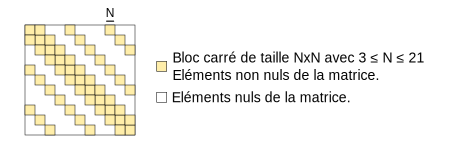
\includegraphics[width=0.7\textwidth]{images/matrices_reservoir.pdf}
      \caption{Matrices utilisées pour la simulation de réservoir.}
      \label{matrice_reservoir}
  \end{center}\end{figure}

 %-------------------------------
 \subsection{Les matrices creuses}
  Les matrices creuses sont des matrices essentiellement composées de zéros.  
  Pour ne pas avoir à stocker tous les zéros, seuls les éléments non
  nuls (NZ) sont stockés. Différents formats de stockage de matrices
  creuses existent comme le COO (\textit{COOrdinate list}) ou le CSR
  (\textit{Compressed Sparse Row}) et permettent d'encoder de
  différentes manières les coordonnées des éléments non nuls.
  Le format a un impact sur la taille de la matrice en mémoire et sur
  l'ordre des accès mémoires.

 %-------------------------------
 \subsection{La programmation GPGPU}
  La programmation GPGPU consiste à détourner l'utilisation du
  processeur graphique (GPU), pour lui faire effectuer des calculs
  généralistes. Pour cela, nous devons écrire 
  un code, aussi appelé Noyau (\textit{Kernel}), dans un langage exprimant le
  parallélisme (CUDA pour une carte NVIDIA ou OpenCL
  pour la portabilité). Dans ces langages, le
  parallélisme est exprimé sous la forme de \textit{Thread}, un \textit{Thread}
  représente une instance du Noyau auquel on a donné un identifiant.
  Les \textit{Threads} sont organisés en groupes appelés \textit{Warp}, les \textit{Threads}
  d'un même \textit{Warp} sont totalement synchrones.

  Le GPU, à l'inverse du CPU, est surtout composé d'unités de calcul.
  Cela permet de pouvoir faire s'exécuter un grand nombre de \textit{Threads} en
  parallèle.
  %Regardons plus en détail l'architecture des unités de
  %calcul du GPU sur la figure \ref{sp_arch}.
  
  %   (-_-)   %
  %\begin{figure}\begin{center}
  %    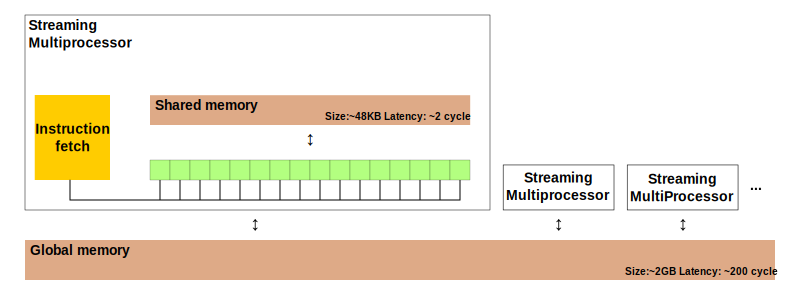
\includegraphics[width=\textwidth]{images/streaming_processor.pdf}
  %    \caption{Architecture d'un Streaming Processor.}
  %    \label{sp_arch}
  %\end{center}\end{figure}
  
  Avec l'architecture Fermi de NVIDIA, 
  le GPU est composé d'unités SIMD appelées Streaming Processor (SP), ces
  unités sont capable à un instant T d'exécuter N instructions
  identiques sur N données potentiellement différentes, avec N la
  taille d'un \textit{Warp}, 32 dans le cas de CUDA.

  Il existe deux types de mémoire sur GPU :
  \begin{itemize}
  \item la mémoire partagée (\textit{shared memory}), de petite taille et avec une faible
    latence, partagée entre les \textit{Threads} d'un bloc.
  \item la mémoire globale (\textit{global memory}), commune à tous les \textit{Threads}, mais avec une
    latence élevée qui peut être masquée par l'utilisation
    d'un grand nombre de \textit{Threads}.
  \end{itemize}

  Les accès à
  la mémoire globale présentent une contrainte, pour que les 32
  instructions puissent s'exécuter en parallèle, les 32 données doivent
  être présentes dans le SP, or la mémoire globale ne peut envoyer que 128 octets à
  la fois (soit 32 float), les \textit{Threads} doivent donc accéder aux données contiguës en
  mémoire, on appelle cela faire des accès coalescés. Si les données sont
  réutilisées plusieurs fois, il peut être avantageux de les placer
  dans la mémoire locale (\textit{shared memory}) pour minimiser la latence et aussi pour pouvoir faire
  des accès désordonnés à la mémoire locale plutôt qu'à la mémoire globale.

  Dans le cas du SpMV ($Ax=b$), seul les données du vecteur multiplicatif $x$ sont
  lues plusieurs fois et de manière désordonnés, elles peuvent être donc
  mises en cache

  %=========================================================
  \section{Étude}
  %=========================================================
  %-------------------------------
  \subsection{Proposition}
   Maintenant que nous en connaissons un peu plus sur l'architecture des
   GPU, nous pouvons étudier l'écriture d'un produit matrice/vecteur efficace.
   Pour cela nous devons choisir un format de représentation adéquat des matrices
   creuses. En effet, sur GPU, l'ordre des accès mémoire est un élément essentiel à prendre
   en compte si nous souhaitons l'exploiter au maximum de ses capacités. Pour cela
   le format de stockage des matrices creuse doit nous permettre d'accéder
   correctement à la mémoire. Nous allons donc tester plusieurs
   formats existants pour trouver le meilleur. Puis, si possible, créer
   un nouveau format moins générique qui prendra en compte la structure
   particulière de nos matrices. 


   %-------------------------------
   \subsection{Expérimentation des principaux formats existants}
    La station de test est composée de 3 Tesla C2050 (puissance crête :
    1030 Gflops et 3 Go de mémoire pour un GPU) et de 2 Xeon X5570 (4 coeurs,
    2.93 GHz pour un CPU).
    
    Les résultats sont exprimés en flops, pour chaque élément non nuls
    de la matrice, nous effectuons une multiplication et une addition, la
    formule pour calculer les flops est donc : $(2 * NNZ) / Temps$, NNZ
    représente le nombre d'éléments non nuls.
    
    Les matrices utilisées sont générées par un programme développé par
    Total et sont représentatives de ce qui est réellement utilisé.
    Les matrices utilisées sont les suivantes :
    \begin{itemize}
      \item 64000 x 64000 avec des blocs de taille 8 x 8 et un total de 0.8 million de non zéros ;
      \item 128000 x 128000 avec des blocs de taille 16 x 16 et un total de 14 million de non zéros ;
      \item 216000 x 216000 avec des blocs de taille 8 x 8 et un total de 12 million de non zéros ;
      \item 432000 x 432000 avec des blocs de taille 16 x 16 et un total de 47 million de non zéros.
    \end{itemize}
    Nous les nommons respectivement 20\_8, 20\_16, 30\_8 et 30\_16.


    Avec ces matrices, nous testons deux propriétés :
    \begin{itemize}
      \item La scalabilité des Noyaux GPU en fonction du nombre d'éléments non nuls ;
      \item l'influence de la taille des blocs sur les performances.
    \end{itemize}
    
    Pour les tests sur CPU, nous utiliserons la librairie MKL d'Intel \cite{MKL} regroupant des
    routines d'algèbres linéaires efficaces. Pour les test sur GPU, nous utiliserons
    le framework CUDA de NVIDIA \cite{CUDA}. Les temps de transfert entre le CPU et le GPU ne sont
    pas pris en compte, ces transferts peuvent être éliminés par le portage complet sur GPU des
    autres opérations du solveur linéaire. La parallélisation sur plusieurs coeurs de calculs
    se fera via StarPU \cite{AugThiNamWac11CCPE}, il s'occupera des transferts mémoires entre le CPU
    et le GPU ainsi que de la gestion des contextes CUDA. Le découpage de la matrice reste à notre charge.
    
    
    %-------------------------------
    \subsection{CSR : Compressed Sparse Row}
    
    %   (-_-)   %
    \begin{figure}\begin{center}
        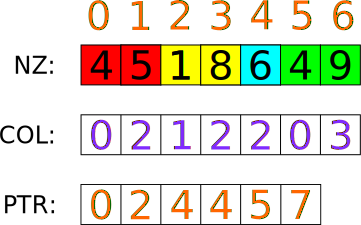
\includegraphics[width=0.7\textwidth]{images/CSR.pdf}
        \caption{Compressed Sparse Row}
        \label{csr_info}
    \end{center}\end{figure}
    
    Les éléments non nuls (NZ) sont stockés par ligne, pour chaque élément nous
    avons sa colonne (COL) et sa ligne doit être calculée en utilisant
    PTR. Le tableau PTR correspond à l'indice dans NZ du premier élément
    d'une ligne. (Fig. \ref{csr_info})
    
    L'implémentation du CSR sur GPU n'est pas évidente, pour avoir des accès mémoire coalescés
    à la matrice, il faut que les \textit{Threads} d'un même \textit{Warp} travail sur la même ligne, or cela
    pose deux problèmes :
    \begin{itemize}
      \item un problème d'accès concurrent au vecteur résultat, ce problème peut être réglé par une
        réduction du résultat de chaque \textit{Thread} à la fin de chaque ligne, une technique efficace existe
        en CUDA \cite{HarrisReductionCUDA} ;
      \item une charge de travail par \textit{Warp} insuffisante, pour nos matrices les
        \textit{Threads} d'un \textit{Warp} n'ont qu'entre 2 et 4 opérations à effectuer.
    \end{itemize}
    Malgré ces problèmes, le choix d'un \textit{Warp} par ligne reste plus efficace que le choix d'un
    \textit{Thread} par ligne.

    Nous avons comparé notre version avec les version implémentés dans
    cuSPARSE \cite{cuSPARSE} et Cusp \cite{Cusp}, nous obtenons les mêmes
    performances.
    

    Sur la figure \ref{spmv_result} nous pouvons remarquer qu'un SpMV sur un GPU atteint
    entre 10 et 19 Gflops alors que les 8 coeurs du CPU n'atteignent que 4 Gflops.

    
    Dans nos cas, quelque soit la taille de la matrice, les performances sur CPU sont
    équivalentes. Par contre, sur le GPU, la taille des blocs a un impact sur les performances.
    Cela provient du fait que les accès mémoire à l'intérieur d'un \textit{Warp} deviennent coalescés,
    pour une taille de bloc égale à 8 il faut lire 4 segments mémoires potentiellement non coalescés du vecteur
    multiplicatif alors qu'avec une taille de bloc égale à 16, nous n'avons plus que 2 segments à lire.
        
    
    %-------------------------------
    \subsection{JAD : JAgged Diagonale storage ou JDS}
    %   (-_-)   %
    \begin{figure}\begin{center}
        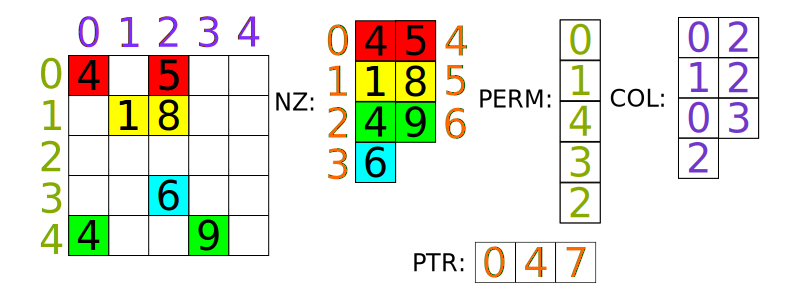
\includegraphics[width=0.7\textwidth]{images/JAD.pdf}
        \caption{JAgged Diagonale storage}
        \label{jad_info}
    \end{center}\end{figure}
 
    La JAD \cite{LiSa10GAPILS} consiste d'abord à ``pousser'' tous les éléments vers la gauche,
    puis à trier les lignes par ordre décroissant d'éléments non nuls. Les permutions résultant
    du tri sont stockées dans un tableau PERM.
    Les données sont stockées par colonne (Fig. \ref{jad_info}).
    
    Le JAD est un format adapté aux machines vectorielles, pour le cas du SpMV les
    données contiguës en mémoire représente toujours une écriture dans des données
    contiguës en mémoire et sans recouvrement. Son implémentation sur GPU est plutôt
    simple, il suffit d'attribuer un \textit{Thread} par ligne de la matrice, les données étant
    stockées par colonne, les accès mémoire à la matrice sont coalescés.
    
    
    Les performances du format JAD varie entre 18 et 25 Gflops sur GPU (Fig. \ref{spmv_result}).
    Pour ce format, la taille des blocs n'a pas d'importance, les matrices 20\_16 
    et 30\_8 obtiennent quasiment les même performances malgré la différence de taille de blocs.
    
    Ce format est donc environ 1,5 fois plus efficace que le CSR pour nos matrices.
    Mais dans les tests que nous avons
    effectuées, nous n'avons pas pris en compte le temps de permutation des vecteurs, celui-ci
    pouvant être évité par un réordonnancement des inconnues dans la résolution.

    Le format ELL \cite{VOFG10Improving} est un format proche du JAD, mais au lieu de trier les lignes
    par nombre d'éléments non nuls, le format ELL fait du remplissage en ajoutant des éléments nuls en fin
    de ligne pour avoir des lignes de même longueur, ce format est à privilégier au JAD dans le cas d'une
    matrice régulière. Ce format est utilisé par Cusp \cite{Cusp}.


 %-------------------------------
 \subsection{BCSR : Block Compress Sparse Row}
   %   (-_-)   %
   \begin{figure}\begin{center}
       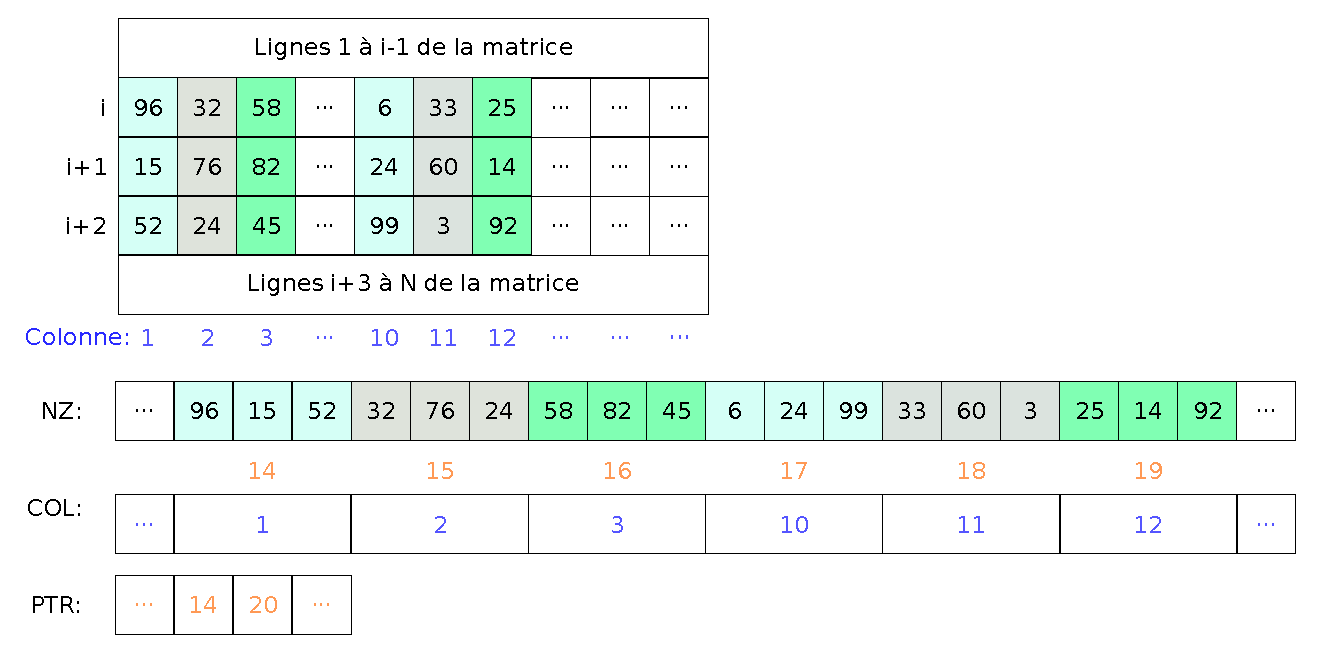
\includegraphics[width=0.8\textwidth]{images/BCSR.pdf}
       \caption{Block Compressed Sparse Row, exemple d'une ligne contenant 2 blocs de taille 3x3}
       \label{bcsr_info}
   \end{center}\end{figure}
    %   (-_-)   %
    \begin{figure}\begin{center}
        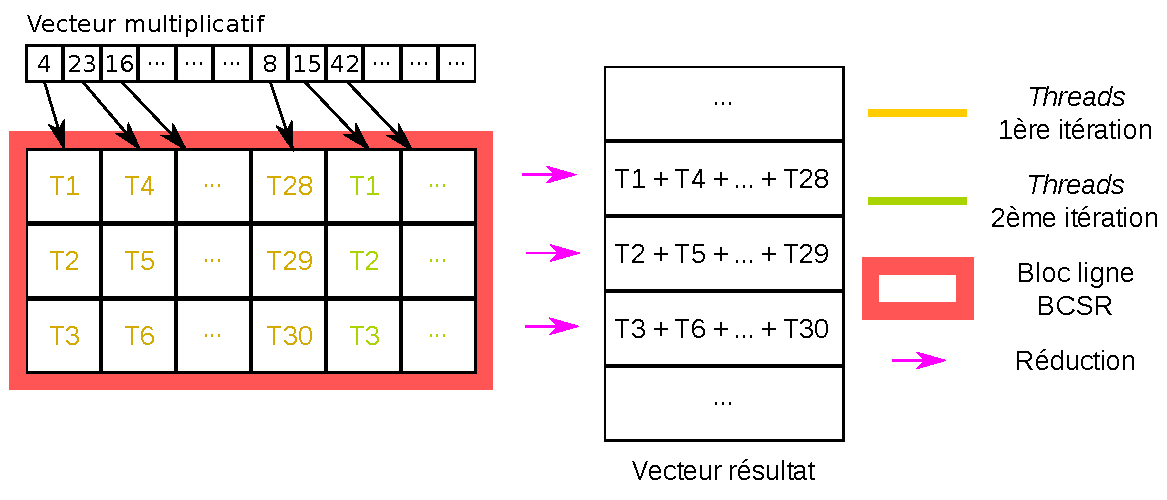
\includegraphics[width=0.7\textwidth]{images/distrib_bcsr.pdf}
        \caption{Répartition des \textit{Threads} à l'intérieur d'un bloc BCSR de taille 3x3
          sur GPU, les \textit{Threads} 31 et 32 sont exclus du travail.}
        \label{distrib_bcsr}
    \end{center}\end{figure}
   
   Le BCSR est une adaptation du format CSR pour nos matrices. Il reprend le
   principe du CSR mais stocke des blocs de lignes (Fig. \ref{bcsr_info}). Cette structure est
   naturellement adaptée à la structure de nos matrices et va permettre d'utiliser un
   \textit{Warp} par bloc-ligne de manière plus efficace que le CSR.
   L'implémentation classique du BCSR correspond à un stockage continue des blocs par ligne \cite{ChSi10MDAS},
   nous proposons de stocker les coefficients non nuls \textbf{par colonne} et
   de \textbf{stocker de manière scalaire} l'indice de chaque colonne: ainsi le produit d'un bloc-ligne
   par le vecteur multiplicatif peut se paralléliser indépendamment de la structure en bloc du
   bloc-ligne.


   \subsubsection{Implémentation sur GPU du SpMV}
    \label{impl_bcsr}
    L'utilisation des blocs nous permet d'attribuer un \textit{Warp} par bloc tout en garantissant
    assez de travail pour chaque \textit{Thread}. A l'intérieur du 
    bloc-ligne les \textit{Threads} peuvent lire des données continues en mémoire et grâce au
    stockage par colonne, ils peuvent partagés en mémoire locale les données
    du vecteur multiplicatif (Fig. \ref{distrib_bcsr}). Lorsque la hauteur $h$ d'un bloc n'est pas
    un diviseur de 32, seuls les \textit{Threads} ayant un identifiant inférieur au plus grand
    multiple de $h$ inférieur à 32 effectuent des calculs, les autres ne font rien (Algo. \ref{bcsr_code}).
    Par exemple, dans la figure \ref{distrib_bcsr}, les \textit{Threads} 31 et 32 sont inutilisés.
    A la fin d'un bloc ligne, une réduction dans la vecteur résultat doit être effectuée, le stockage
    par colonne permet d'effectuer plus efficacement la somme des produits de la ligne dans le 
    vecteur résultat. En effet, à l'intérieur d'un bloc-ligne, un \textit{Thread} ne participe qu'à une seule
    ligne ce qui réduit le nombre d'étapes pour effectuer la réduction finale. Pour faciliter l'identification
    des \textit{Threads} appartenant à un même \textit{Warp}, nous avons décider d'utiliser la première dimension de
    \textit{threadIdx} comme identifiant à l'intérieur d'un \textit{Warp} et la deuxième dimension de
    \textit{threadIdx} (+ l'identifiant du \textit{Block} CUDA) comme identifiant de \textit{Warp}.
    

\begin{algorithm}
 \caption{Pseudo-code du SpMV au format BCSR.}
 \label{bcsr_code}
 \SetAlgoLined
 \Entree{NZ, COL, PTR pour la matrice, X le vecteur multiplicatif}
 \Sortie{Y le vecteur résultat}
 Const WARP\_SIZE = 32\;
 Const BLOCK\_SIZE = la taille des blocs de la matrice\;
 Const colonne\_par\_itération = (WARP\_SIZE/BLOCK\_SIZE)\;
 \Si{threadIdx.x > colonne\_par\_itération*BLOCK\_SIZE}{
   \CommentSty{// Les threads inutilisés du warp}\\
   \Retour
 }

 Let ligne\_courante = blockIdx.x + threadIdx.y\;
 Let colonne = threadIdx.x $\backslash$ BLOCK\_SIZE\;
 Let ligne\_locale = threadIdx.x \% BLOCK\_SIZE\;
 Let sum\_tmp = 0\;
 Let i = (PTR[ligne\_courante]+colonne)*BLOCK\_SIZE+ligne\_locale\;
 Let j = PTR[ligne\_courante]+colonne\;
 \Tq{j < PTR[ligne\_courante+1]}{
  sum\_tmp += NZ[i] * X[COL[j]]\;
  i += colonne\_par\_itération\ * BLOCK\_SIZE\;
  j += colonne\_par\_itération\;
 }
 Réduction des sum\_tmp -> Y[ligne\_courante+ligne\_locale]\;
\end{algorithm}
    
    \subsubsection{Résultats}
    %   (-_-)   %
    \begin{figure}\begin{center}
        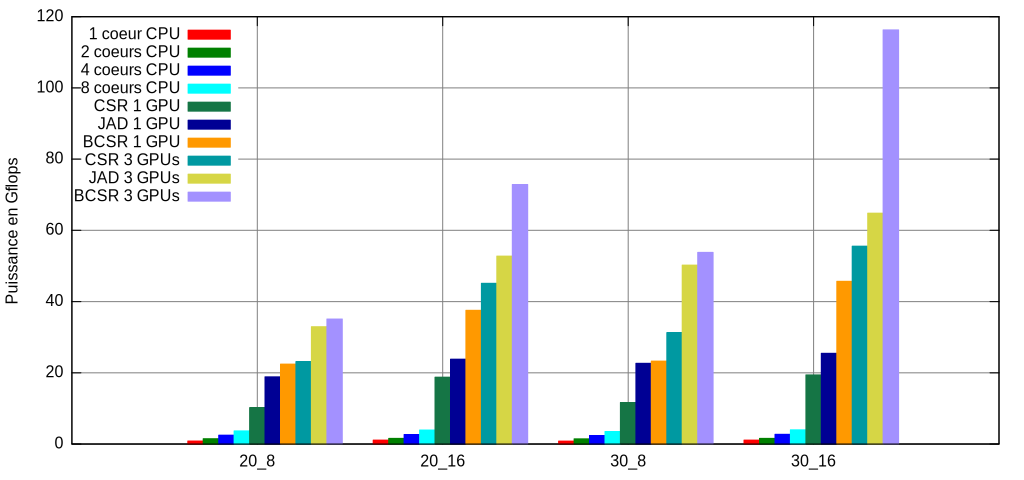
\includegraphics[width=1.05\textwidth]{images/SPMV.pdf}
        \caption{Performance du SpMV sur les différents formats de stockage des matrices}
        \label{spmv_result}
    \end{center}\end{figure}
   
    Les performances sur un GPU sont doublées par rapport au format CSR.
    Ainsi nous atteignons de l'ordre de 45 Gflops sur un GPU alors que la 
    puissance obtenue sur 8 coeurs CPU n'est que de 5 Gflops (cas 30\_16 de la figure \ref{spmv_result}).
    Sur 3 GPUs, nous atteignons même 120 Gflops, soit 24 fois le résultat obtenu avec les
    CPUs de la station.
    Cette différence de performance avec le format CSR s'explique par trois améliorations :
    \begin{itemize}
      \item Le stockage par colonne qui permet le partage du vecteur multiplicatif ;
      \item une écriture coalescée dans le vecteur résultat à la fin d'une ligne ;
      \item une plus grande charge de travail par Warp.
    \end{itemize}

  %-------------------------------
  \subsection{Autres formats}
   Parmi les autres formats qui existent, nous pouvons citer :
   \begin{itemize}
     \item CSC : format identique au CSR mais le stockage se fait par colonne,
       le stockage complet de la matrice par colonne ne permet pas d'écrire un SpMV sur GPU à
       cause des accès concurrent en écriture au vecteur résultat ;
     \item DIA : seuls les diagonales contenant au moins un élément non nul sont stockées, dans notre
       cas les diagonales des bords de bloc ne contiennent pas assez de valeur, les performances sont
       équivalentes au CSR.
   \end{itemize}

%=========================================================
\section{Conclusion}
%=========================================================
 Le produit matrice/vecteur creux présente de nombreuses difficultés
 pour être porté sur GPU. De par son irrégularité, nous sommes
 obligés d'utiliser des tableaux d'indirections pour accéder aux
 éléments. Or l'utilisation de ces tableaux sur GPU est très coûteuse,
 c'est pour cela que nous avons cherché un format de matrices creuses 
 pour la simulation de réservoir adapté aux GPUs.

 Dans la littérature, nous avons trouvé le format JAD imaginé pour les
 anciennes machines vectorielles \cite{Blelloch93segmentedoperations},
 ce format s'adapte très bien aux GPUs modernes.
 
 Notre recherche d'un format adapté à nos matrices, nous
 a conduits au format BCSR dans lequel les blocs sont stockés par
 colonne. Malgré les bonnes performances du BCSR, les performances
 crêtes du GPU sont loin d'être atteintes. Cela s'explique par le fait
 que nous faisons trois accès mémoire, dont un indirect, pour seulement deux
 opérations.

 Parmi les formats \textit{standards} que nous
 avons essayés, le ELL et le JAD se sont montrés efficaces mais moins
 que le BCSR. Dans le cas général, l'utilisation du format JAD 
 % ou du format sliced ELL\cite{MoLo10ATSMV}
 sur GPU  offrira de meilleurs performances que le format CSR.

 Maintenant que le SpMV est implémenté sur GPU, nous devons porter le
 reste des opérations du solveur sur GPU. Parmi ces opérations nous avons
 la factorisation ILU0 et les résolutions triangulaires, qui requièrent
 une gestion du parallélisme à grain fin. La version actuelle de CUDA
 ne nous permet pas d'implémenter ces deux opérations sur GPU, la 
 prochaine version (CUDA 5) devrait le permettre.

\bibliography{solver_gpu}


\end{document}
